\documentclass[11pt,a4paper]{article}

% Image mode: pdf.
% Image paths stay relative. In PDF mode, place same-basename PDF conversions
% of the chapter SVG files in the assets/ directory beside this source.

\usepackage{iftex}
\ifPDFTeX
  \PackageError{handout}{This template requires XeTeX or Tectonic}{Compile with xelatex or tectonic.}
\fi

\usepackage[a4paper,top=18mm,bottom=20mm,left=20mm,right=20mm,headsep=6mm]{geometry}
\usepackage{fontspec}
\usepackage{xeCJK}
\usepackage{amsmath}
\usepackage{unicode-math}

% Font settings are intentionally visible in the generated .tex file.
% These defaults target the macOS machine used for the released PDF.
% Change the family names when compiling on another system.
\setmainfont{Songti TC}
\setsansfont{Heiti TC}
\setmonofont{Menlo}
\setCJKmainfont{Songti TC}
\setCJKsansfont{Heiti TC}
\setCJKmonofont{Heiti TC}
\setmathfont{STIX Two Math}
\XeTeXlinebreaklocale "zh"
\XeTeXlinebreakskip=0pt plus 1pt

\usepackage{xcolor}
\definecolor{HandoutBlue}{HTML}{215A91}
\definecolor{HandoutBlueLight}{HTML}{EEF5FC}
\definecolor{HandoutGreen}{HTML}{39715A}
\definecolor{HandoutGreenLight}{HTML}{EFF8F3}
\definecolor{HandoutGold}{HTML}{8A641C}
\definecolor{HandoutGoldLight}{HTML}{FFF8E8}
\definecolor{HandoutInk}{HTML}{253142}
\definecolor{HandoutMuted}{HTML}{667085}

\usepackage{graphicx}
\makeatletter
% Pandoc 3 emits an accessibility `alt` key for raster/PDF images. Older
% graphicx releases do not know that key, so accept it without changing layout.
\@ifundefined{KV@Gin@alt}{\define@key{Gin}{alt}{}}{}
\newsavebox\pandoc@box
\newcommand*\pandocbounded[1]{%
  \sbox\pandoc@box{#1}%
  \Gscale@div\@tempa{\textheight}{\dimexpr\ht\pandoc@box+\dp\pandoc@box\relax}%
  \Gscale@div\@tempb{\linewidth}{\wd\pandoc@box}%
  \ifdim\@tempb\p@<\@tempa\p@\let\@tempa\@tempb\fi
  \ifdim\@tempa\p@<\p@\scalebox{\@tempa}{\usebox\pandoc@box}%
  \else\usebox{\pandoc@box}%
  \fi
}
\makeatother
\usepackage{float}
\floatplacement{figure}{H}
% Pandoc uses LTcaptype=none for uncaptioned longtables. The caption package
% expects that name to exist as a counter even though it is never displayed.
\newcounter{none}
\usepackage{caption}
\captionsetup[figure]{labelformat=empty,labelsep=none,font=small}

\usepackage{booktabs,longtable,array,calc}
\usepackage{etoolbox}
\makeatletter
\patchcmd\longtable{\par}{\if@noskipsec\mbox{}\fi\par}{}{}
\makeatother

\usepackage[most]{tcolorbox}
\tcbuselibrary{breakable,skins}
\newtcolorbox{HandoutLearningMap}{
  enhanced,breakable,colback=HandoutBlueLight,colframe=HandoutBlue,
  boxrule=0.8pt,arc=1.5mm,left=3mm,right=3mm,top=2mm,bottom=2mm,
  before skip=8pt,after skip=10pt
}
\newtcolorbox{HandoutWorkedExample}{
  enhanced,breakable,colback=HandoutGreenLight,colframe=HandoutGreen,
  boxrule=0.65pt,arc=1.5mm,left=3mm,right=3mm,top=2mm,bottom=2mm,
  before skip=8pt,after skip=10pt
}
\newtcolorbox{HandoutSelfCheck}{
  enhanced,breakable,colback=HandoutGoldLight,colframe=HandoutGold,
  boxrule=0.65pt,arc=1.5mm,left=3mm,right=3mm,top=2mm,bottom=2mm,
  before skip=8pt,after skip=10pt
}

\usepackage{titlesec}
\titleformat{\section}{\sffamily\bfseries\Large\color{HandoutBlue}}{}{0pt}{}
\titleformat{\subsection}{\sffamily\bfseries\large\color{HandoutInk}}{}{0pt}{}
\titleformat{\subsubsection}{\sffamily\bfseries\normalsize\color{HandoutInk}}{}{0pt}{}
\titlespacing*{\section}{0pt}{1.4em}{0.55em}
\titlespacing*{\subsection}{0pt}{1.15em}{0.45em}
\titlespacing*{\subsubsection}{0pt}{0.9em}{0.35em}
\setcounter{secnumdepth}{-\maxdimen}

\usepackage{hyperref}
\usepackage{bookmark}
\IfFileExists{xurl.sty}{\usepackage{xurl}}{}
\urlstyle{same}
\hypersetup{
  colorlinks=true,
  linkcolor=HandoutBlue,
  urlcolor=HandoutBlue,
  citecolor=HandoutBlue,
  pdftitle={數B3-1 正弦函數與週期性現象},
  pdfsubject={數學},
  pdfcreator={Pandoc with the HighSchooContent LaTeX template}
}

\setlength{\parindent}{0pt}
\setlength{\parskip}{0.55em plus 0.15em minus 0.1em}
\setlength{\emergencystretch}{3em}
\setlength{\LTpre}{0.5em}
\setlength{\LTpost}{0.5em}
\renewcommand{\arraystretch}{1.18}
\providecommand{\tightlist}{%
  \setlength{\itemsep}{0pt}\setlength{\parskip}{0pt}}
\pagestyle{plain}


\begin{document}

\begin{tcolorbox}[
  enhanced,colback=white,colframe=HandoutBlue,boxrule=1.1pt,arc=2mm,
  borderline west={3pt}{0pt}{HandoutBlue},left=5mm,right=4mm,top=4mm,bottom=4mm
]
{\sffamily\small\bfseries\color{HandoutBlue}學生講義}\par
{\sffamily\bfseries\LARGE\color{HandoutInk}數B3-1 正弦函數與週期性現象}\par
\vspace{0.35em}{\large 用弧度連結圓周運動與正弦圖形，以振幅、週期和平移描述重複變化}\par
\vspace{0.45em}{\small\color{HandoutMuted}%
科目：數學
\quad 課程：普通高中數學B 第三冊
\quad 版本：學生版｜核心＋理解
\quad 校訂：2026-08-31
}\par
\vspace{0.25em}{\small\color{HandoutMuted}範圍：114 學年度數學B第三冊第 1 章；弧度量、弧長與扇形面積、週期性現象、正弦函數圖形、平移伸縮與週期模型}\par
\end{tcolorbox}


\begin{HandoutLearningMap}

\subsection{本章問題與能力}\label{ux672cux7ae0ux554fux984cux8207ux80fdux529b}

\begin{enumerate}
\def\labelenumi{\arabic{enumi}.}
\tightlist
\item
  角度如何直接表示圓弧長度與扇形面積？
\item
  重複出現的事件如何用週期描述？
\item
  單位圓上的點如何生成正弦函數圖形？
\item
  振幅、週期、中線與相位如何控制週期模型？
\item
  如何從摩天輪、聲波或溫度資料建立正弦模型，並判斷模型的適用範圍？
\end{enumerate}

本章路徑：弧度量 → 弧長與扇形面積 → 週期 → 單位圓與正弦圖形 → 圖形變換 → 週期模型。

\end{HandoutLearningMap}

\section{0. 本章用途與實際應用：把旋轉與重複變化寫成同一種數學語言}\label{ux672cux7ae0ux7528ux9014ux8207ux5be6ux969bux61c9ux7528ux628aux65cbux8f49ux8207ux91cdux8907ux8b8aux5316ux5bebux6210ux540cux4e00ux7a2eux6578ux5b78ux8a9eux8a00}

鐘針、摩天輪與旋轉機械都沿圓周運動。圓周上的位置投影到鉛直方向後，會形成正弦形狀的週期變化。弧度量使「轉過多少角」直接等於「弧長除以半徑」，因此圓周幾何、角速度與正弦函數能使用同一個變數。

聲音的振動、日照時數、潮汐與季節溫度也會反覆起伏。週期模型用中線表示平均水準、振幅表示偏離平均的最大量、週期表示一次循環所需時間、相位表示循環的起始狀態。這些參數讓圖形可以轉回具體的高度、頻率、時間與範圍。

真實資料常含有天氣、地形、阻力或多個頻率的影響。單一正弦函數描述主要循環；殘差則保留其他因素造成的差異。模型的用途是建立可檢查的近似。

\section{1. 弧度量}\label{ux5f27ux5ea6ux91cf}

\subsection{1.1 弧度的定義}\label{ux5f27ux5ea6ux7684ux5b9aux7fa9}

半徑為 \(r\) 的圓中，圓心角 \(\theta\) 所對的弧長為 \(s\)。\textbf{弧度量}定義為

\[
\theta=\frac{s}{r}.
\]

當 \(s=r\) 時，\(\theta=1\)，稱為 \textbf{1 弧度}。弧度是兩個長度的比值，因此沒有長度單位。書寫 \(\theta=2\) 時，角度單位預設為弧度；度數則保留 \(^\circ\) 符號。

\begin{figure}
\centering
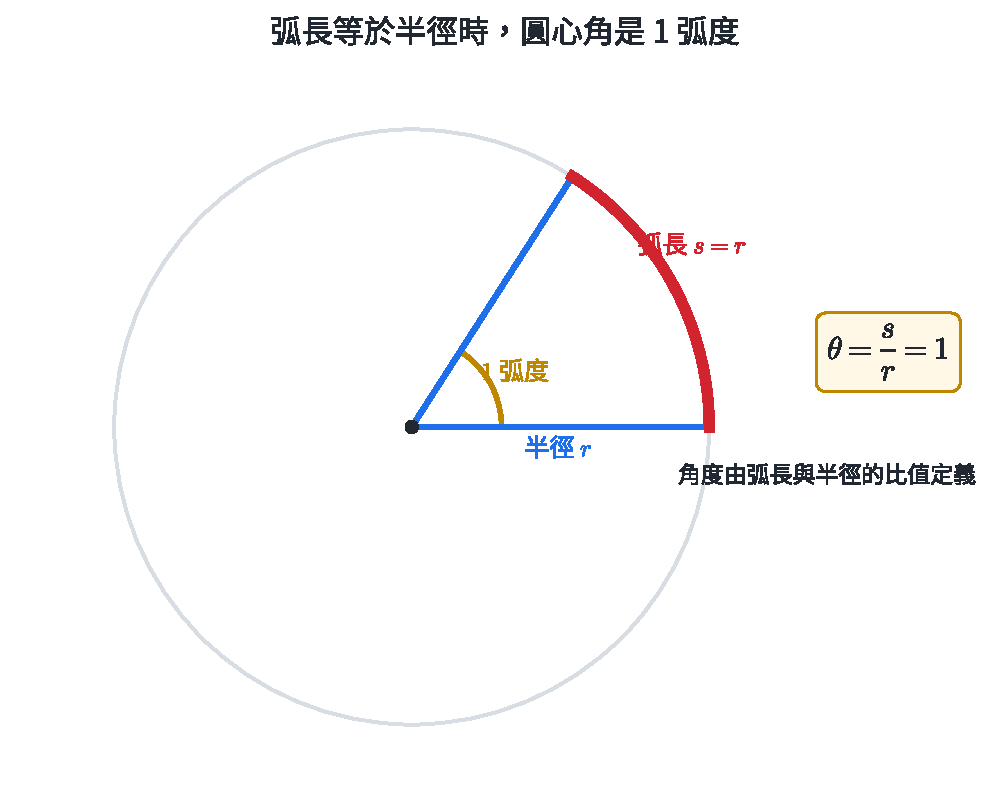
\includegraphics[width=0.88\linewidth,height=\textheight,keepaspectratio,alt={弧長等於半徑時的 1 弧度}]{assets/數B3-1-一弧度定義.pdf}
\caption{弧長等於半徑時的 1 弧度}
\end{figure}

一整圈的弧長是 \(2\pi r\)，所以

\[
\text{一整圈}=\frac{2\pi r}{r}=2\pi\text{ 弧度}.
\]

由 \(360^\circ=2\pi\) 可得

\[
180^\circ=\pi,\qquad 1^\circ=\frac{\pi}{180},\qquad
1\text{ 弧度}=\frac{180^\circ}{\pi}.
\]

因此，兩種角度制的換算規則為

\[
\alpha^\circ=\alpha\cdot\frac{\pi}{180}\text{ 弧度},
\]

\[
\theta\text{ 弧度}=\theta\cdot\frac{180}{\pi}{}^\circ.
\]

計算機輸入弧度時使用 RAD 模式；輸入度數時使用 DEG 模式。角度模式不同會直接改變三角函數值。

\begin{figure}
\centering
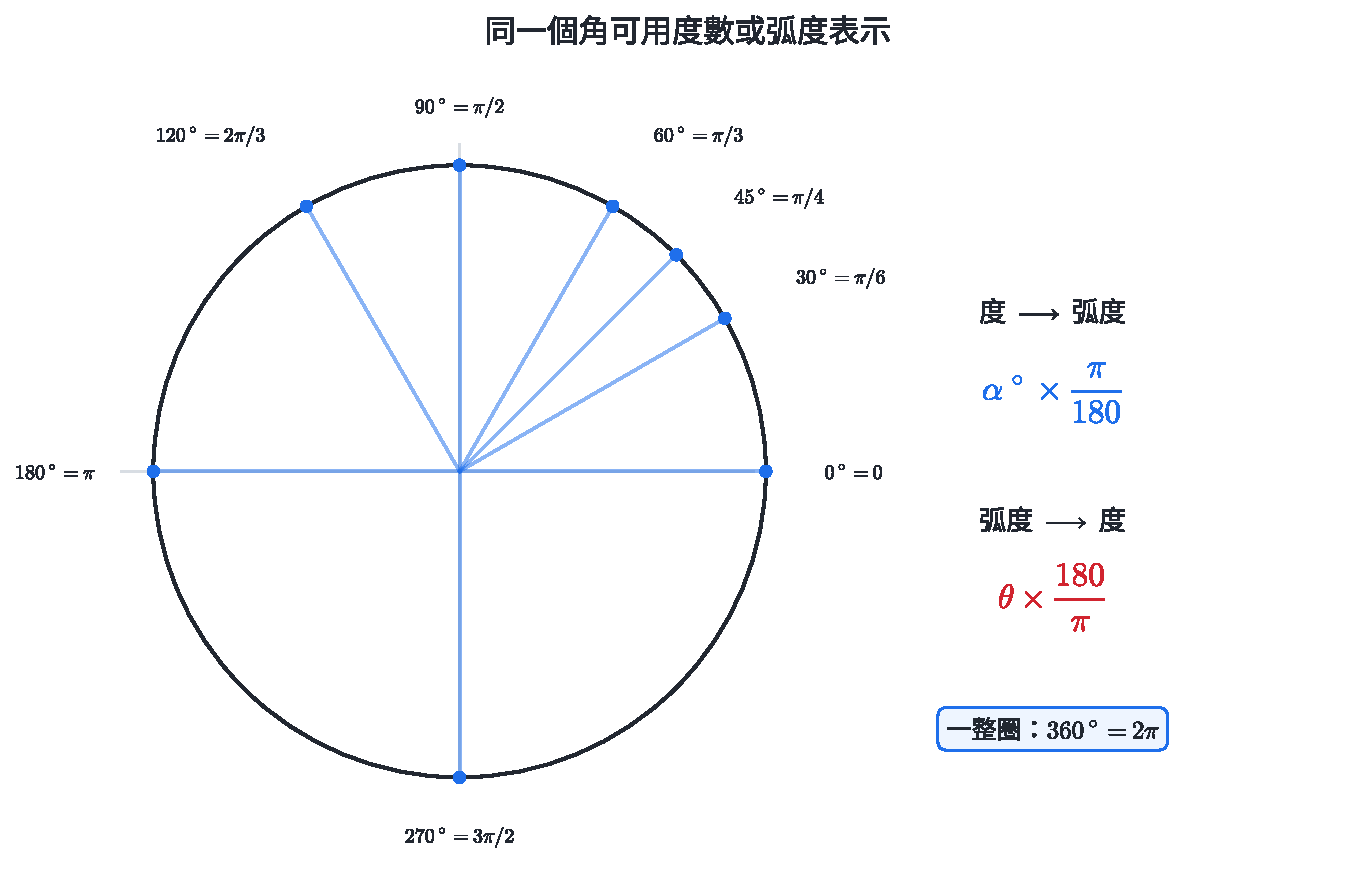
\includegraphics[width=0.94\linewidth,height=\textheight,keepaspectratio,alt={常用角的度數與弧度對照}]{assets/數B3-1-度與弧度對照.pdf}
\caption{常用角的度數與弧度對照}
\end{figure}

兩個角若終邊相同，稱為\textbf{同界角}。以弧度表示時，它們相差整數圈：

\[
\theta+2k\pi,\qquad k\in\mathbb Z.
\]

這個規則可把很大的正角或負角化到 \([0,2\pi)\)，再判斷象限與三角比。

\subsection{例 1｜度數與弧度互換}\label{ux4f8b-1ux5ea6ux6578ux8207ux5f27ux5ea6ux4e92ux63db}

將 \(225^\circ\) 化為弧度，並將 \(-\dfrac{7\pi}{6}\) 化為度數。

\[
225^\circ=225\cdot\frac{\pi}{180}=\frac{5\pi}{4}.
\]

\[
-\frac{7\pi}{6}=-\frac{7\pi}{6}\cdot\frac{180}{\pi}{}^\circ=-210^\circ.
\]

換算後的方向與角度大小保持一致：\(225^\circ\) 超過半圈，\(-210^\circ\) 表示順時針轉過 \(210^\circ\)。

\subsection{例 2｜化簡同界角並求三角比}\label{ux4f8b-2ux5316ux7c21ux540cux754cux89d2ux4e26ux6c42ux4e09ux89d2ux6bd4}

求 \(\dfrac{25\pi}{6}\) 在 \([0,2\pi)\) 的同界角、所在象限及其正弦值。

先減去兩圈：

\[
\frac{25\pi}{6}-4\pi=\frac{\pi}{6}.
\]

\(\pi/6\) 位於第一象限，因此

\[
\sin\frac{25\pi}{6}=\sin\frac{\pi}{6}=\frac12.
\]

\subsection{例 3｜由旋轉圈數求弧度}\label{ux4f8b-3ux7531ux65cbux8f49ux5708ux6578ux6c42ux5f27ux5ea6}

轉盤逆時針轉 \(0.4\) 圈，轉角為

\[
0.4\times2\pi=\frac{4\pi}{5}.
\]

若接著順時針轉 \(\pi/5\)，淨轉角為

\[
\frac{4\pi}{5}-\frac{\pi}{5}=\frac{3\pi}{5}.
\]

圈數乘上 \(2\pi\) 可直接轉成弧度；方向由正負號表示。

\subsection{1.2 分節練習}\label{ux5206ux7bc0ux7df4ux7fd2}

\begin{enumerate}
\def\labelenumi{\arabic{enumi}.}
\tightlist
\item
  將 \(150^\circ\) 與 \(-315^\circ\) 化為弧度。
\item
  將 \(\dfrac{7\pi}{12}\) 與 \(-\dfrac{4\pi}{3}\) 化為度數。
\item
  求 \(\dfrac{29\pi}{6}\) 在 \([0,2\pi)\) 的同界角、所在象限及正弦、餘弦值。
\item
  求 \(-\dfrac{11\pi}{4}\) 在 \([0,2\pi)\) 的同界角及所在象限。
\item
  一個輪子逆時針轉 \(2.75\) 圈後，再順時針轉 \(\dfrac{3\pi}{2}\)。求淨轉角的弧度量。
\end{enumerate}

\subsection{1.3 分節練習解析}\label{ux5206ux7bc0ux7df4ux7fd2ux89e3ux6790}

\begin{enumerate}
\def\labelenumi{\arabic{enumi}.}
\tightlist
\item
  \[150^\circ=\frac{5\pi}{6},\qquad -315^\circ=-\frac{7\pi}{4}.\]
\item
  \[\frac{7\pi}{12}=105^\circ,\qquad -\frac{4\pi}{3}=-240^\circ.\]
\item
  \[\frac{29\pi}{6}-4\pi=\frac{5\pi}{6}.\]
  這是第二象限角，故
  \[\sin\frac{29\pi}{6}=\frac12,\qquad
  \cos\frac{29\pi}{6}=-\frac{\sqrt3}{2}.\]
\item
  加上兩圈：
  \[-\frac{11\pi}{4}+4\pi=\frac{5\pi}{4}.\]
  所以同界角為 \(5\pi/4\)，位於第三象限。
\item
  \(2.75\) 圈是 \(11\pi/2\)，故淨轉角為
  \[\frac{11\pi}{2}-\frac{3\pi}{2}=4\pi.\]
\end{enumerate}

弧度把轉角、半徑與弧長連在同一條比例式上；機械旋轉、鐘針移動與地球表面距離都可直接沿用這個定義。

\section{2. 弧長與扇形面積}\label{ux5f27ux9577ux8207ux6247ux5f62ux9762ux7a4d}

\subsection{2.1 公式與推導}\label{ux516cux5f0fux8207ux63a8ux5c0e}

設扇形半徑為 \(r\)、圓心角為 \(\theta\) 弧度。標準扇形取 \(0\le\theta\le2\pi\)，它占整圓的比例是 \(\theta/(2\pi)\)。因此

\[
s=2\pi r\cdot\frac{\theta}{2\pi}=r\theta,
\]

\[
A=\pi r^2\cdot\frac{\theta}{2\pi}
=\frac12r^2\theta.
\]

再代入 \(s=r\theta\)，得到

\[
A=\frac12rs.
\]

\begin{figure}
\centering
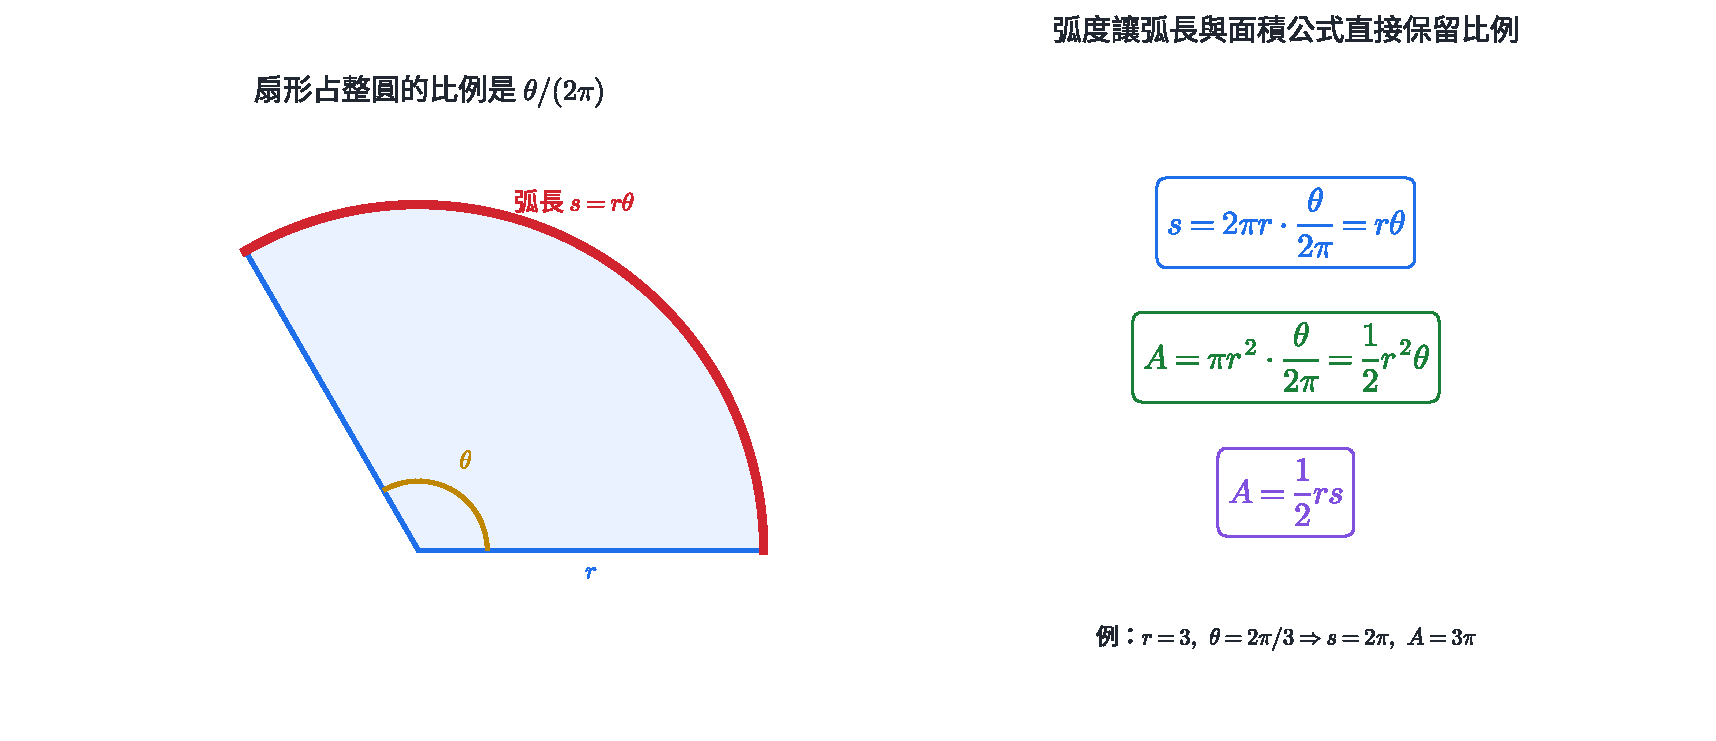
\includegraphics[width=0.96\linewidth,height=\textheight,keepaspectratio,alt={弧長與扇形面積由整圓比例推得}]{assets/數B3-1-弧長與扇形面積.pdf}
\caption{弧長與扇形面積由整圓比例推得}
\end{figure}

這三式的角度 \(\theta\) 使用弧度。題目若給度數，先乘上 \(\pi/180\)。單位由半徑決定：\(s\) 與 \(r\) 使用相同長度單位，\(A\) 使用相應的平方單位。

環形扇形可視為兩個同角度扇形的差。外半徑 \(R\)、內半徑 \(r\)、圓心角 \(\theta\) 時，

\[
A=\frac12(R^2-r^2)\theta,
\]

\[
P=(R+r)\theta+2(R-r).
\]

周長式的前半段是內外兩段圓弧，後半段是兩段徑向線段。

旋轉路程題可讓累積轉角 \(\theta\) 超過 \(2\pi\)，此時 \(s=r\theta\) 計算多圈累積路程；扇形面積則依題意決定重疊區域計一次或按掃掠次數累計。

\subsection{例 4｜已知半徑與角度}\label{ux4f8b-4ux5df2ux77e5ux534aux5f91ux8207ux89d2ux5ea6}

半徑 \(6\) 公分的扇形，圓心角為 \(5\pi/6\)。求弧長與面積。

\[
s=6\cdot\frac{5\pi}{6}=5\pi\text{ cm},
\]

\[
A=\frac12\cdot36\cdot\frac{5\pi}{6}=15\pi\text{ cm}^2.
\]

它占整圓的 \(5/12\)，弧長與面積都保持這個比例。

\subsection{例 5｜由扇形周長反求角度與面積}\label{ux4f8b-5ux7531ux6247ux5f62ux5468ux9577ux53cdux6c42ux89d2ux5ea6ux8207ux9762ux7a4d}

一個扇形的半徑為 \(5\) 公分，周長為 \(26\) 公分。求圓心角與面積。

\[
2r+s=26\quad\Rightarrow\quad s=16.
\]

\[
\theta=\frac{s}{r}=\frac{16}{5},
\]

\[
A=\frac12rs=40\text{ cm}^2.
\]

\subsection{例 6｜環形扇面的面積與周長}\label{ux4f8b-6ux74b0ux5f62ux6247ux9762ux7684ux9762ux7a4dux8207ux5468ux9577}

一把扇子形成圓心角 \(2\pi/3\) 的環形扇形，外半徑 \(30\) 公分、內半徑 \(12\) 公分。求面積與邊界周長。

\[
A=\frac12(30^2-12^2)\frac{2\pi}{3}=252\pi\text{ cm}^2.
\]

\[
P=(30+12)\frac{2\pi}{3}+2(30-12)=28\pi+36\text{ cm}.
\]

\subsection{例 7｜分針針尖的路程與掃掠面積}\label{ux4f8b-7ux5206ux91ddux91ddux5c16ux7684ux8defux7a0bux8207ux6383ux63a0ux9762ux7a4d}

分針長 \(12\) 公分，經過 \(35\) 分鐘。分針轉角為

\[
\theta=2\pi\cdot\frac{35}{60}=\frac{7\pi}{6}.
\]

針尖路程與掃過面積分別為

\[
s=12\cdot\frac{7\pi}{6}=14\pi\text{ cm},
\]

\[
A=\frac12(12)^2\frac{7\pi}{6}=84\pi\text{ cm}^2.
\]

\begin{figure}
\centering
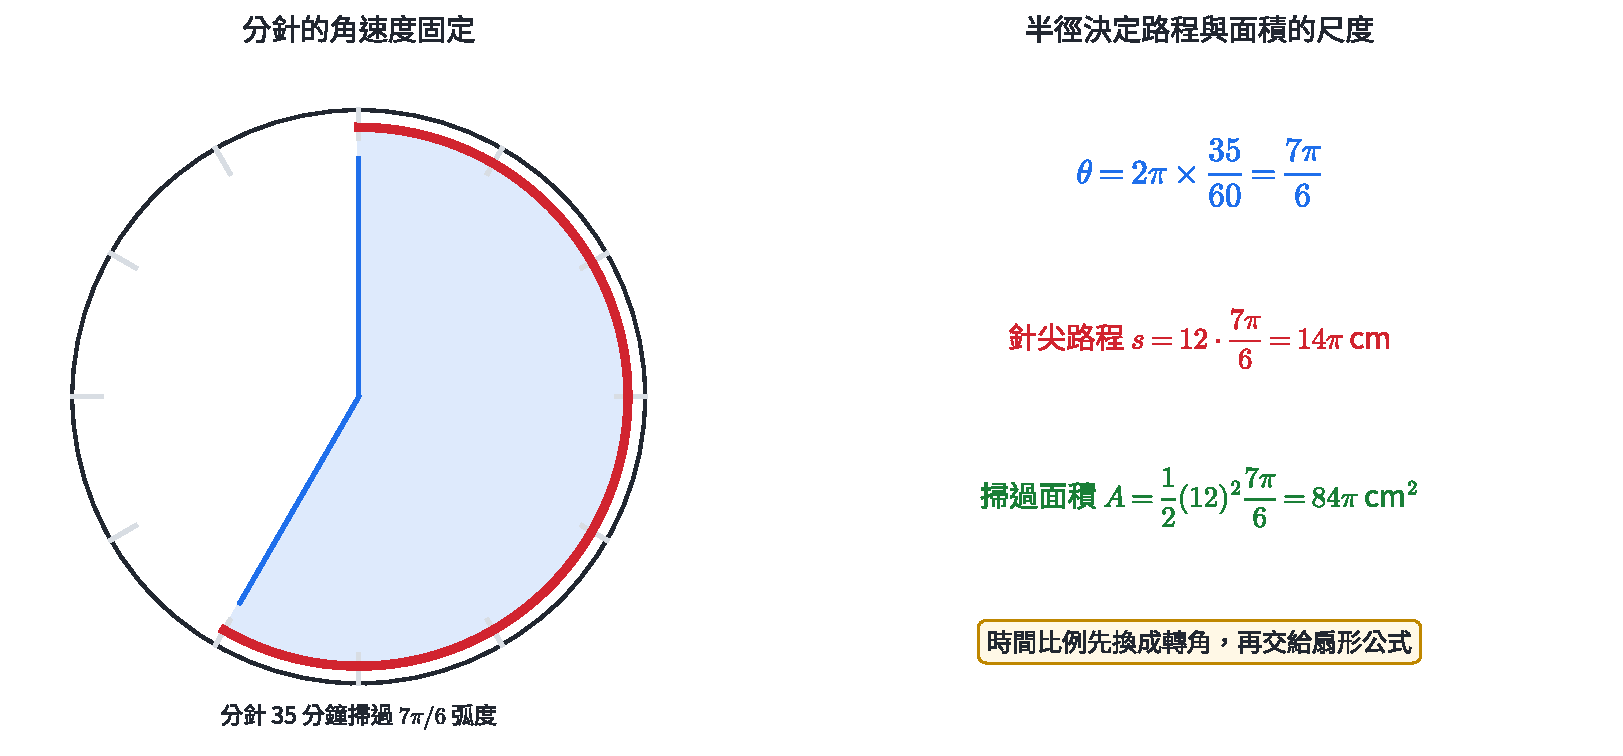
\includegraphics[width=0.95\linewidth,height=\textheight,keepaspectratio,alt={分針的時間比例、轉角、路程與掃掠面積}]{assets/數B3-1-時鐘掃掠.pdf}
\caption{分針的時間比例、轉角、路程與掃掠面積}
\end{figure}

\subsection{2.2 分節練習}\label{ux5206ux7bc0ux7df4ux7fd2-1}

\begin{enumerate}
\def\labelenumi{\arabic{enumi}.}
\tightlist
\item
  半徑 \(8\) 公分、圓心角 \(3\pi/4\) 的扇形，求弧長與面積。
\item
  半徑 \(10\) 公分、圓心角 \(72^\circ\) 的扇形，求弧長與面積。
\item
  一扇形的弧長為 \(15\) 公分，圓心角為 \(2.5\) 弧度。求半徑與面積。
\item
  一扇形的周長為 \(24\) 公分，圓心角為 \(2\) 弧度。求半徑與面積。
\item
  環形扇形的外半徑為 \(10\) 公分、內半徑為 \(6\) 公分、圓心角為 \(\pi/2\)。求面積與邊界周長。
\item
  地球表面兩地沿大圓的弧長約為 \(1110\) 公里，對應地心角為 \(10^\circ\)。以球面近似求地球半徑，四捨五入至十公里。
\end{enumerate}

\subsection{2.3 分節練習解析}\label{ux5206ux7bc0ux7df4ux7fd2ux89e3ux6790-1}

\begin{enumerate}
\def\labelenumi{\arabic{enumi}.}
\tightlist
\item
  \[s=8\cdot\frac{3\pi}{4}=6\pi\text{ cm},\qquad
  A=\frac12(8)^2\frac{3\pi}{4}=24\pi\text{ cm}^2.\]
\item
  \(72^\circ=2\pi/5\)，所以
  \[s=4\pi\text{ cm},\qquad A=20\pi\text{ cm}^2.\]
\item
  \[r=\frac{s}{\theta}=\frac{15}{2.5}=6\text{ cm},\qquad
  A=\frac12rs=45\text{ cm}^2.\]
\item
  \(s=r\theta=2r\)，周長 \(2r+s=4r=24\)，故 \(r=6\) 公分，
  \[A=\frac12r^2\theta=36\text{ cm}^2.\]
\item
  \[A=\frac12(10^2-6^2)\frac{\pi}{2}=16\pi\text{ cm}^2,\]
  \[P=(10+6)\frac{\pi}{2}+2(10-6)=8\pi+8\text{ cm}.\]
\item
  \(10^\circ=\pi/18\)，所以
  \[r=\frac{1110}{\pi/18}=\frac{19980}{\pi}\approx6359.8.\]
  四捨五入至十公里約為 \(6360\) 公里。
\end{enumerate}

弧長公式用於輪帶行程、鐘針路程與地球表面距離；扇形面積用於扇面材料、噴灑區域與旋轉掃掠範圍。

\section{3. 週期性現象}\label{ux9031ux671fux6027ux73feux8c61}

\subsection{3.1 離散循環與連續週期函數}\label{ux96e2ux6563ux5faaux74b0ux8207ux9023ux7e8cux9031ux671fux51fdux6578}

一串離散資料若每隔 \(p\) 項重複，即

\[
a_{n+p}=a_n
\]

對所有允許的索引 \(n\) 成立，則 \(p\) 是一個週期；最小正整數週期稱為\textbf{基本週期}。星期、生肖與整數次方的末位數都可用餘數判定循環位置。

\begin{figure}
\centering
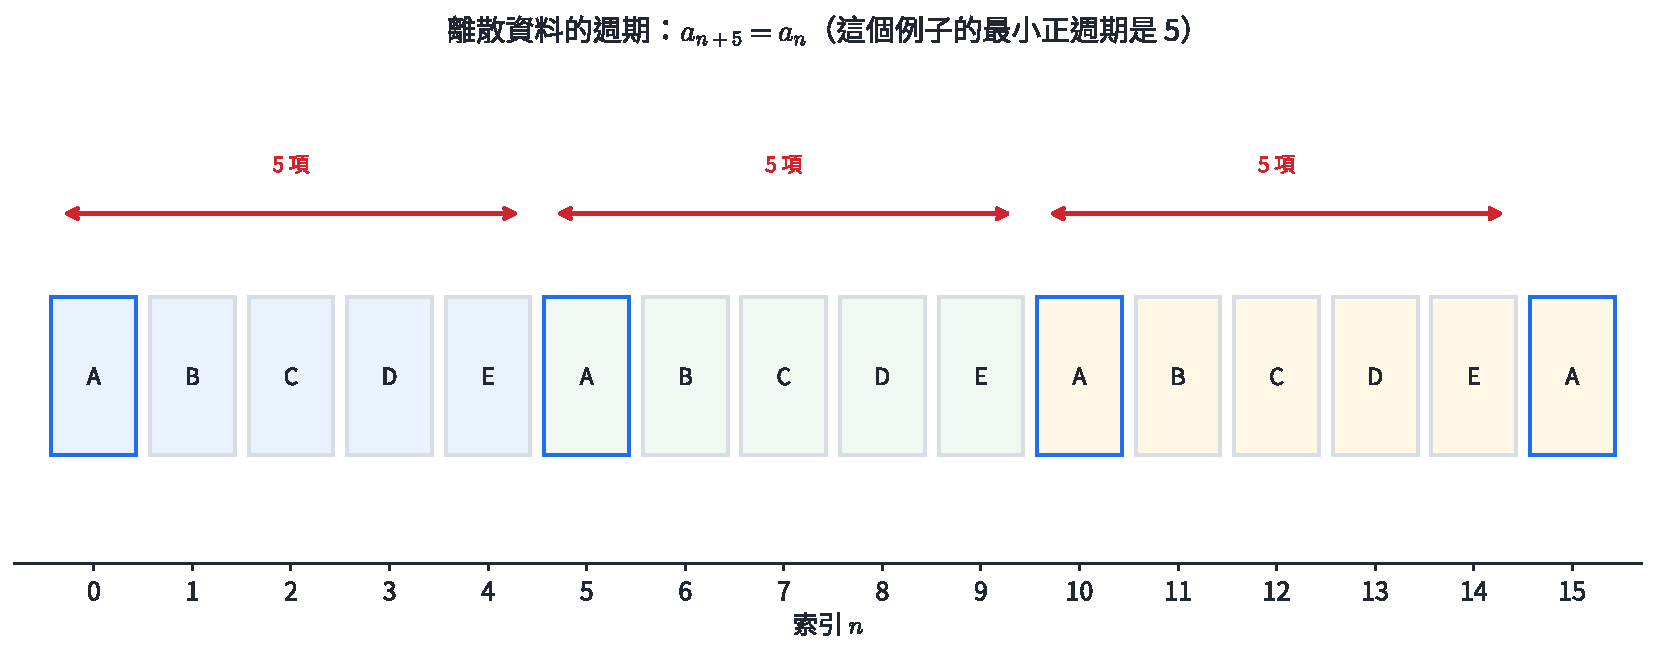
\includegraphics[width=0.95\linewidth,height=\textheight,keepaspectratio,alt={離散序列每 5 項重複一次}]{assets/數B3-1-離散週期.pdf}
\caption{離散序列每 5 項重複一次}
\end{figure}

函數 \(f\) 若存在正數 \(T\)，使定義域內每個適用的 \(x\) 都滿足

\[
f(x+T)=f(x),
\]

則 \(f\) 是\textbf{週期函數}，\(T\) 是它的一個週期。最小正週期稱為\textbf{基本週期}。例如 \(2\pi,4\pi,6\pi,\ldots\) 都是 \(\sin x\) 的週期，其中 \(2\pi\) 是基本週期。

兩個事件若分別每 \(m\) 與 \(n\) 個時間單位發生一次，且目前同時發生，下一次同時發生的等待時間是 \(\operatorname{lcm}(m,n)\)。這是離散週期的同步問題。

觀測資料可呈現近似週期。例如相鄰滿潮時間可能相差 \(12.4\) 小時、\(12.6\) 小時、\(12.3\) 小時。平均間隔可估計主要週期；預測時保留天氣、海岸形狀與天文週期造成的偏差。

\subsection{例 8｜末位數的循環}\label{ux4f8b-8ux672bux4f4dux6578ux7684ux5faaux74b0}

求 \(2^{2026}\) 的個位數。

\(2\) 的正整數次方個位數依次為

\[
2,4,8,6,2,4,8,6,\ldots
\]

基本週期為 \(4\)。因為 \(2026=4\cdot506+2\)，所以第 \(2026\) 項與循環中的第 \(2\) 項相同，個位數是 \(4\)。

\subsection{例 9｜兩個週期事件何時再次同步}\label{ux4f8b-9ux5169ux500bux9031ux671fux4e8bux4ef6ux4f55ux6642ux518dux6b21ux540cux6b65}

甲裝置每 \(18\) 分鐘記錄一次，乙裝置每 \(30\) 分鐘記錄一次。上午 7:00 兩者同時記錄，求下一次同時記錄的時刻。

\[
18=2\cdot3^2,\qquad30=2\cdot3\cdot5,
\]

\[
\operatorname{lcm}(18,30)=2\cdot3^2\cdot5=90.
\]

經過 \(90\) 分鐘後再度同步，因此時刻是上午 8:30。

\subsection{例 10｜由觀測間隔估計主要週期}\label{ux4f8b-10ux7531ux89c0ux6e2cux9593ux9694ux4f30ux8a08ux4e3bux8981ux9031ux671f}

某港口連續三次滿潮時刻，換算成第一天 0:00 起算的時數為 \(2.3,14.8,27.1\)。兩段間隔為

\[
14.8-2.3=12.5,\qquad27.1-14.8=12.3.
\]

以平均值估計主要週期：

\[
T\approx\frac{12.5+12.3}{2}=12.4\text{ 小時}.
\]

這個值適合短期概略預測；正式航行與潮位決策採用當地完整潮汐資料。

\subsection{3.2 分節練習}\label{ux5206ux7bc0ux7df4ux7fd2-2}

\begin{enumerate}
\def\labelenumi{\arabic{enumi}.}
\tightlist
\item
  序列「紅、綠、藍、黃」依序重複，第一項為紅。求第 \(2027\) 項的顏色。
\item
  求 \(3^{100}\) 的個位數。
\item
  兩班接駁車分別每 \(14\) 分鐘與 \(20\) 分鐘發車一次。上午 9:00 同時發車，求下一次同時發車的時刻。
\item
  驗證 \(f(x)=3+2\sin\left(\dfrac{\pi x}{6}\right)\) 以 \(12\) 為週期。
\item
  某地連續四次高水位時刻為起算後 \(1.1,13.6,26.0,38.6\) 小時。估計主要週期，並說明此估計所代表的資料意義。
\end{enumerate}

\subsection{3.3 分節練習解析}\label{ux5206ux7bc0ux7df4ux7fd2ux89e3ux6790-2}

\begin{enumerate}
\def\labelenumi{\arabic{enumi}.}
\tightlist
\item
  基本週期為 \(4\)。因為 \(2027-1=2026\)，而 \(2026\) 除以 \(4\) 餘 \(2\)，故第 \(2027\) 項位於循環索引 \(2\)，也就是第三種顏色「藍」。
\item
  個位數循環為 \(3,9,7,1\)，週期 \(4\)。\(100\) 除以 \(4\) 餘 \(0\)，對應循環第 \(4\) 項，所以個位數為 \(1\)。
\item
  \[\operatorname{lcm}(14,20)=140\text{ 分鐘}.\]
  上午 9:00 加 \(2\) 小時 \(20\) 分鐘，得到上午 11:20。
\item
  \[f(x+12)=3+2\sin\left(\frac{\pi(x+12)}6\right)
  =3+2\sin\left(\frac{\pi x}{6}+2\pi\right)=f(x).\]
  所以 \(12\) 是週期。正弦內角在 \(x\) 增加 \(12\) 時恰增加一整圈，故基本週期也是 \(12\)。
\item
  三段間隔為 \(12.5,12.4,12.6\) 小時，平均為
  \[\frac{12.5+12.4+12.6}{3}=12.5\text{ 小時}.\]
  它描述這四筆資料中的平均重複間隔，可作為主要週期估計；每一次實際高水位仍可能偏離平均時刻。
\end{enumerate}

週期可壓縮長序列、安排同步事件，也能從時間資料抽出主要循環。離散問題常用除法餘數與最小公倍數；連續模型則以 \(f(x+T)=f(x)\) 檢查。

\section{4. 正弦函數的圖形}\label{ux6b63ux5f26ux51fdux6578ux7684ux5716ux5f62}

\subsection{4.1 單位圓生成正弦圖形}\label{ux55aeux4f4dux5713ux751fux6210ux6b63ux5f26ux5716ux5f62}

在單位圓上，從正 \(x\) 軸逆時針轉過 \(x\) 弧度，到達點

\[
P=(\cos x,\sin x).
\]

\(P\) 的縱坐標就是 \(\sin x\)。當角度 \(x\) 連續增加，把每個角度與對應高度畫成點 \((x,\sin x)\)，便得到函數 \(y=\sin x\)。

\begin{figure}
\centering
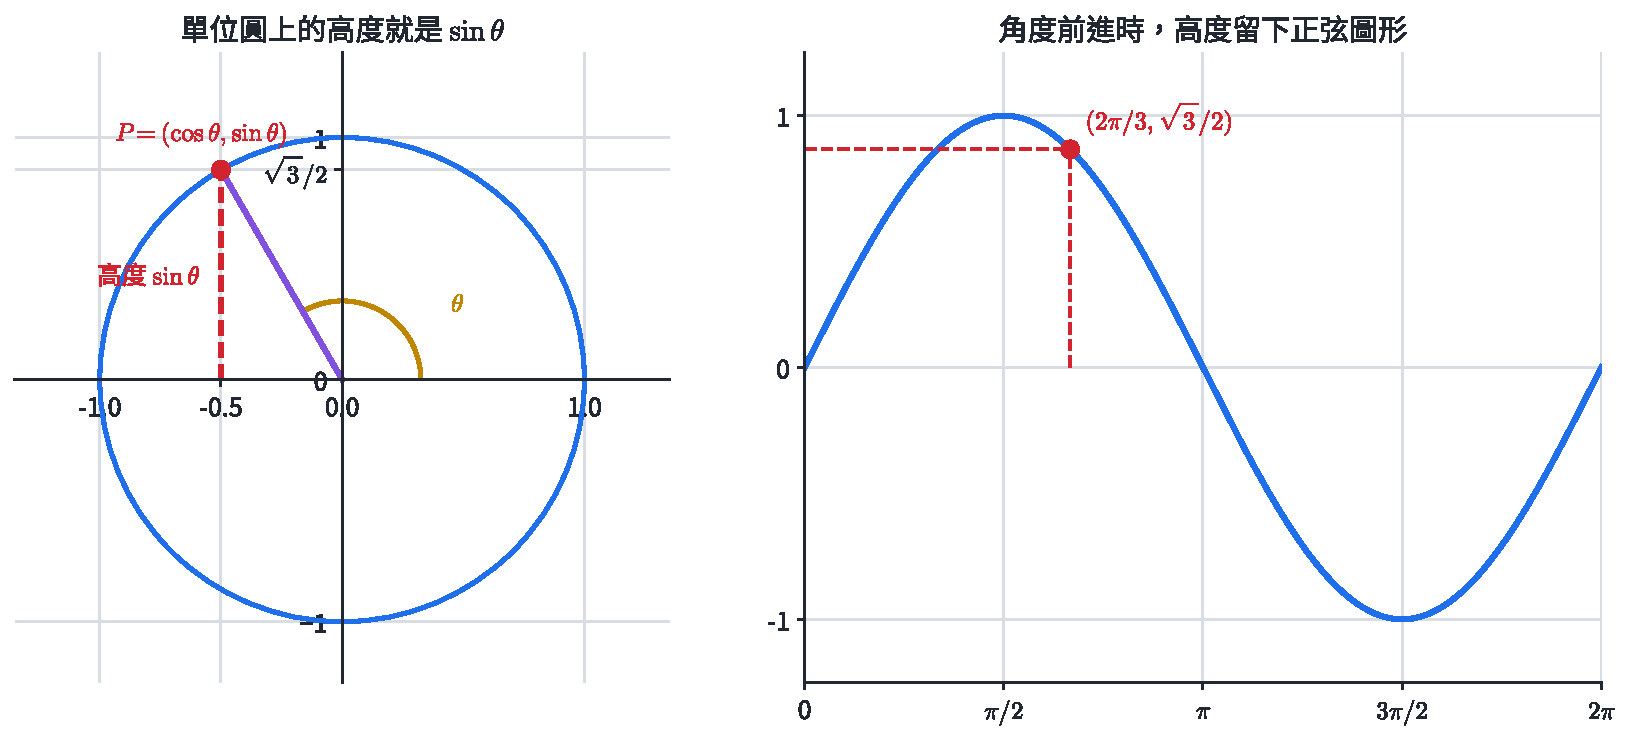
\includegraphics[width=0.96\linewidth,height=\textheight,keepaspectratio,alt={單位圓高度生成正弦函數值}]{assets/數B3-1-單位圓與正弦.pdf}
\caption{單位圓高度生成正弦函數值}
\end{figure}

單位圓直接給出正弦函數的核心性質：

\begin{itemize}
\tightlist
\item
  定義域：所有實數 \(\mathbb R\)。
\item
  值域：\([-1,1]\)，因為單位圓的縱坐標介於 \(-1\) 與 \(1\)。
\item
  基本週期：\(2\pi\)，因為轉一整圈回到同一點，\(\sin(x+2\pi)=\sin x\)。
\item
  奇函數：\(\sin(-x)=-\sin x\)，圖形以原點為對稱中心。
\item
  零點：\(x=k\pi\)。
\item
  最高點：\(x=\pi/2+2k\pi\)，函數值為 \(1\)。
\item
  最低點：\(x=3\pi/2+2k\pi\)，函數值為 \(-1\)。
\end{itemize}

其中 \(k\in\mathbb Z\)。

\begin{figure}
\centering
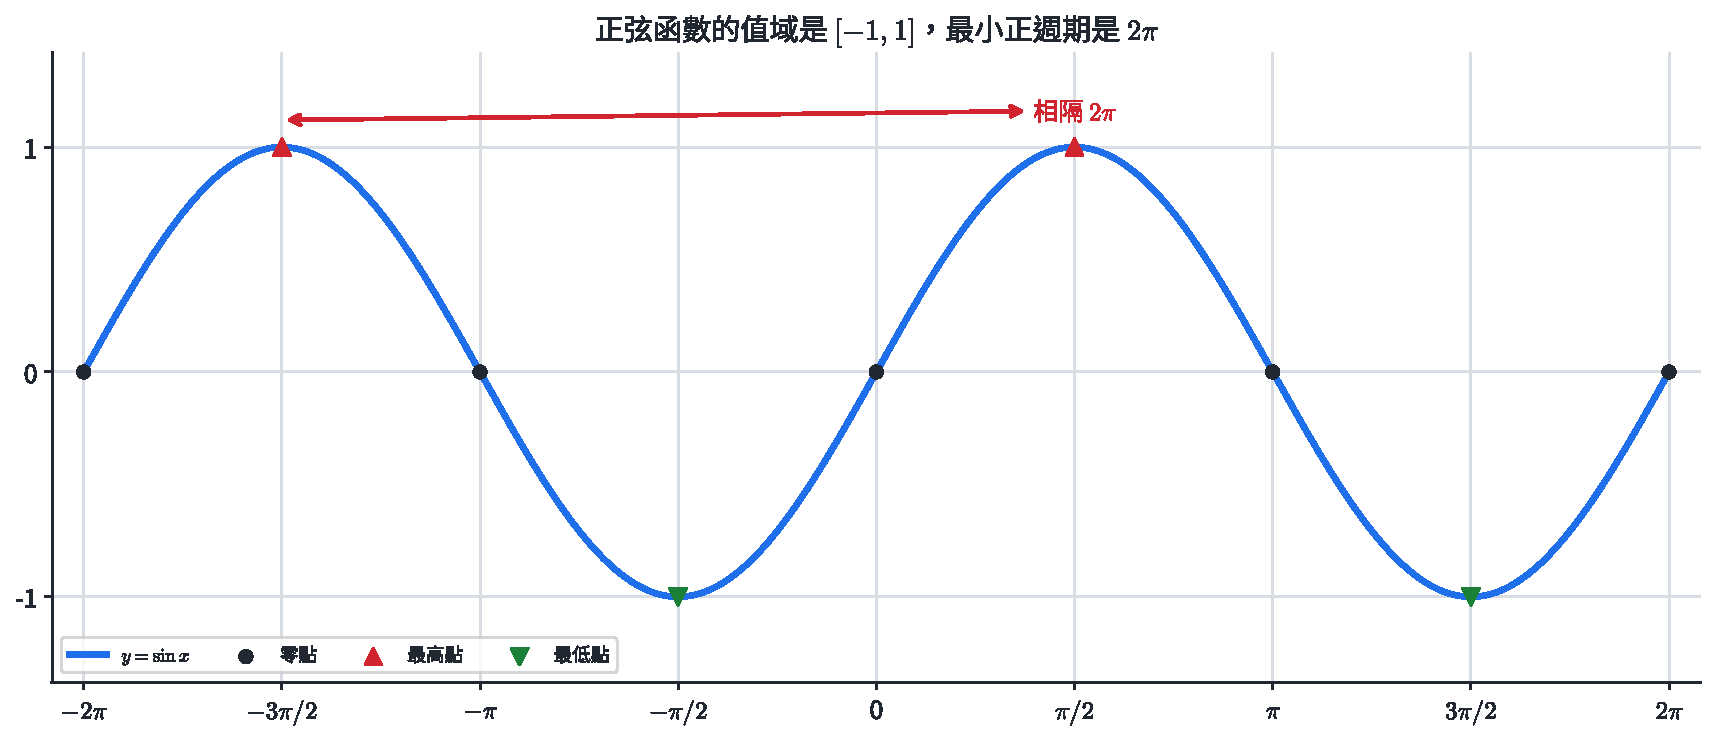
\includegraphics[width=0.97\linewidth,height=\textheight,keepaspectratio,alt={正弦函數的零點、最高點、最低點與週期}]{assets/數B3-1-正弦關鍵點.pdf}
\caption{正弦函數的零點、最高點、最低點與週期}
\end{figure}

正弦函數在

\[
\left[-\frac\pi2+2k\pi,\frac\pi2+2k\pi\right]
\]

隨 \(x\) 增加而上升；在

\[
\left[\frac\pi2+2k\pi,\frac{3\pi}2+2k\pi\right]
\]

隨 \(x\) 增加而下降。這可由單位圓上的縱坐標變化讀出。

\subsection{4.2 用圖形解正弦方程與不等式}\label{ux7528ux5716ux5f62ux89e3ux6b63ux5f26ux65b9ux7a0bux8207ux4e0dux7b49ux5f0f}

在限定區間內解 \(\sin x=c\)，可畫水平線 \(y=c\)，交點的橫坐標就是解。解 \(\sin x\ge c\) 時，找出正弦曲線位於水平線上方的區間，並依不等號決定端點是否納入。

\begin{figure}
\centering
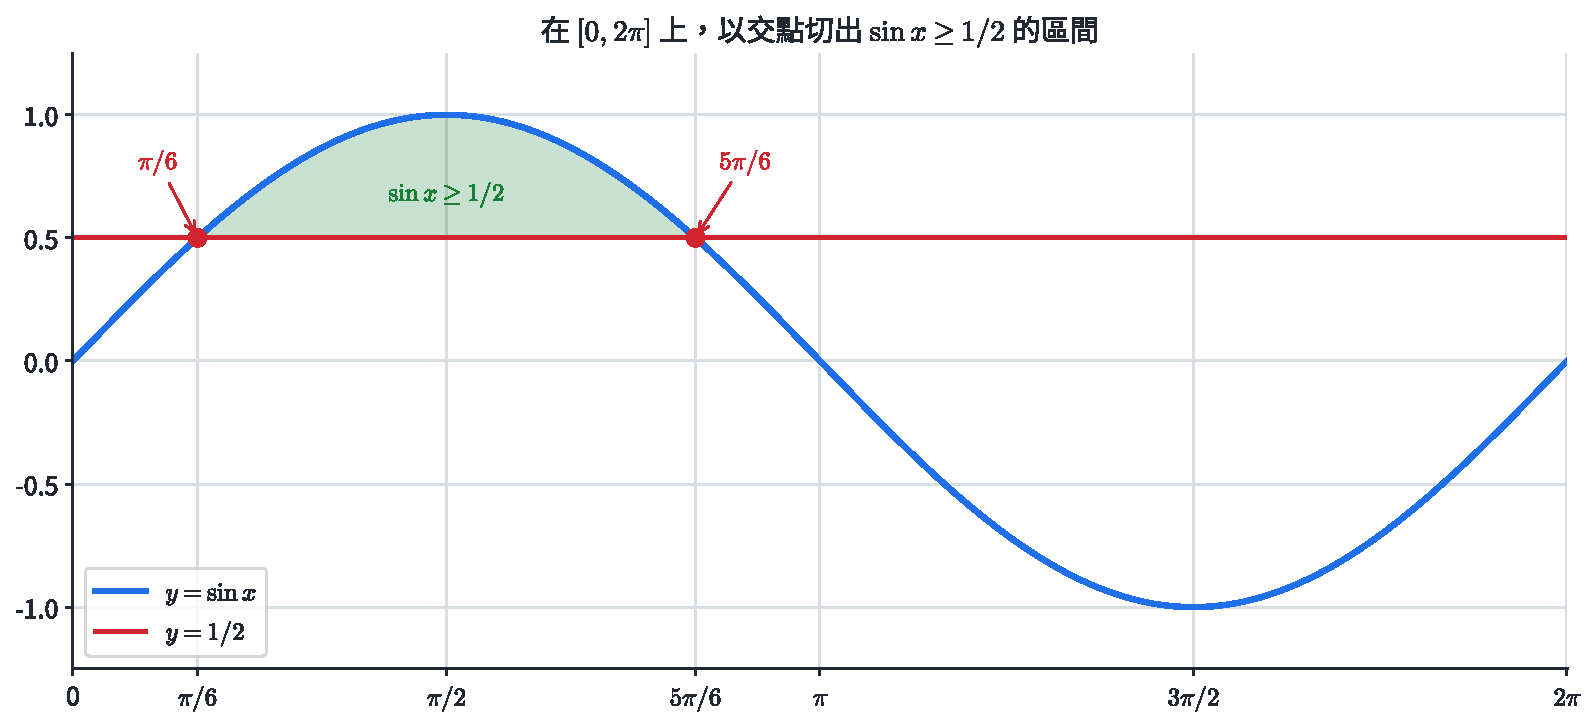
\includegraphics[width=0.94\linewidth,height=\textheight,keepaspectratio,alt={由水平線交點解正弦方程與不等式}]{assets/數B3-1-正弦方程與不等式.pdf}
\caption{由水平線交點解正弦方程與不等式}
\end{figure}

\subsection{例 11｜大角度的函數值與圖形狀態}\label{ux4f8b-11ux5927ux89d2ux5ea6ux7684ux51fdux6578ux503cux8207ux5716ux5f62ux72c0ux614b}

求 \(\sin\dfrac{17\pi}{6}\)，並判斷圖形在該點附近是上升或下降。

\[
\frac{17\pi}{6}-2\pi=\frac{5\pi}{6},\qquad
\sin\frac{17\pi}{6}=\frac12.
\]

\(5\pi/6\) 位於 \([\pi/2,3\pi/2]\) 的下降區間，所以圖形在此點附近下降。

\subsection{例 12｜以關鍵點畫圖}\label{ux4f8b-12ux4ee5ux95dcux9375ux9edeux756bux5716}

在 \([-\pi,2\pi]\) 畫 \(y=\sin x\)。先列關鍵點：

\[
\begin{array}{c|rrrrrrr}
x&-\pi&-\pi/2&0&\pi/2&\pi&3\pi/2&2\pi\\ \hline
\sin x&0&-1&0&1&0&-1&0
\end{array}
\]

依序以平滑曲線連接。曲線在零點穿越 \(x\) 軸，在 \(\pi/2\) 達最高點，在 \(-\pi/2\) 與 \(3\pi/2\) 達最低點。

\subsection{例 13｜解正弦方程}\label{ux4f8b-13ux89e3ux6b63ux5f26ux65b9ux7a0b}

在 \([0,2\pi]\) 解 \(\sin x=\sqrt3/2\)。

單位圓上縱坐標為 \(\sqrt3/2\) 的點位於第一、第二象限，參考角為 \(\pi/3\)，所以

\[
x=\frac\pi3,\quad\frac{2\pi}{3}.
\]

\subsection{例 14｜解正弦不等式}\label{ux4f8b-14ux89e3ux6b63ux5f26ux4e0dux7b49ux5f0f}

在 \([0,2\pi]\) 解 \(\sin x<-1/2\)。

邊界為 \(x=7\pi/6,11\pi/6\)。正弦曲線在兩交點之間位於 \(y=-1/2\) 下方，所以

\[
\frac{7\pi}{6}<x<\frac{11\pi}{6}.
\]

\subsection{4.3 分節練習}\label{ux5206ux7bc0ux7df4ux7fd2-3}

\begin{enumerate}
\def\labelenumi{\arabic{enumi}.}
\tightlist
\item
  寫出 \(y=\sin x\) 的定義域、值域、基本週期與對稱性。
\item
  求 \(\sin(-5\pi/6)\) 與 \(\sin(13\pi/2)\)。
\item
  列出 \([-2\pi,\pi]\) 內 \(y=\sin x\) 的全部零點。
\item
  列出 \([0,4\pi]\) 內 \(y=\sin x\) 的全部最高點與最低點橫坐標。
\item
  在 \([0,2\pi]\) 解 \(\sin x=-\sqrt2/2\)。
\item
  在 \([0,2\pi]\) 解 \(\sin x\ge\sqrt3/2\)。
\end{enumerate}

\subsection{4.4 分節練習解析}\label{ux5206ux7bc0ux7df4ux7fd2ux89e3ux6790-3}

\begin{enumerate}
\def\labelenumi{\arabic{enumi}.}
\tightlist
\item
  定義域為 \(\mathbb R\)，值域為 \([-1,1]\)，基本週期為 \(2\pi\)。因 \(\sin(-x)=-\sin x\)，它是奇函數，圖形以原點為對稱中心。
\item
  \[\sin\left(-\frac{5\pi}{6}\right)=-\frac12.\]
  又 \(13\pi/2-6\pi=\pi/2\)，所以 \(\sin(13\pi/2)=1\)。
\item
  零點為 \(x=k\pi\)。落在區間內的是 \(-2\pi,-\pi,0,\pi\)。
\item
  最高點橫坐標為 \(\pi/2,5\pi/2\)；最低點橫坐標為 \(3\pi/2,7\pi/2\)。
\item
  縱坐標為 \(-\sqrt2/2\) 的單位圓點在第三、第四象限，故
  \[x=\frac{5\pi}{4},\frac{7\pi}{4}.\]
\item
  邊界解為 \(x=\pi/3,2\pi/3\)；曲線在兩點之間位於水平線上方，且包含端點：
  \[\frac\pi3\le x\le\frac{2\pi}{3}.\]
\end{enumerate}

正弦圖形把圓周位置轉成時間曲線。先標零點、最高點、最低點與週期，再判讀方程、區間與變化方向，可保留角度和函數值的幾何關係。

\section{5. 正弦圖形的平移、伸縮與週期模型}\label{ux6b63ux5f26ux5716ux5f62ux7684ux5e73ux79fbux4f38ux7e2eux8207ux9031ux671fux6a21ux578b}

\subsection{5.1 從母圖到一般模型}\label{ux5f9eux6bcdux5716ux5230ux4e00ux822cux6a21ux578b}

以 \(y=\sin x\) 為母圖：

\begin{itemize}
\tightlist
\item
  \(y=\sin x+d\)：向上平移 \(d\)；中線由 \(y=0\) 變成 \(y=d\)。
\item
  \(y=\sin(x-C)\)：向右平移 \(C\)。
\item
  \(y=A\sin x\)，\(A>0\)：縱坐標乘以 \(A\)；振幅為 \(A\)。
\item
  \(y=\sin(Bx)\)，\(B>0\)：橫向尺度縮為原來的 \(1/B\)；基本週期為 \(2\pi/B\)。
\end{itemize}

\begin{figure}
\centering
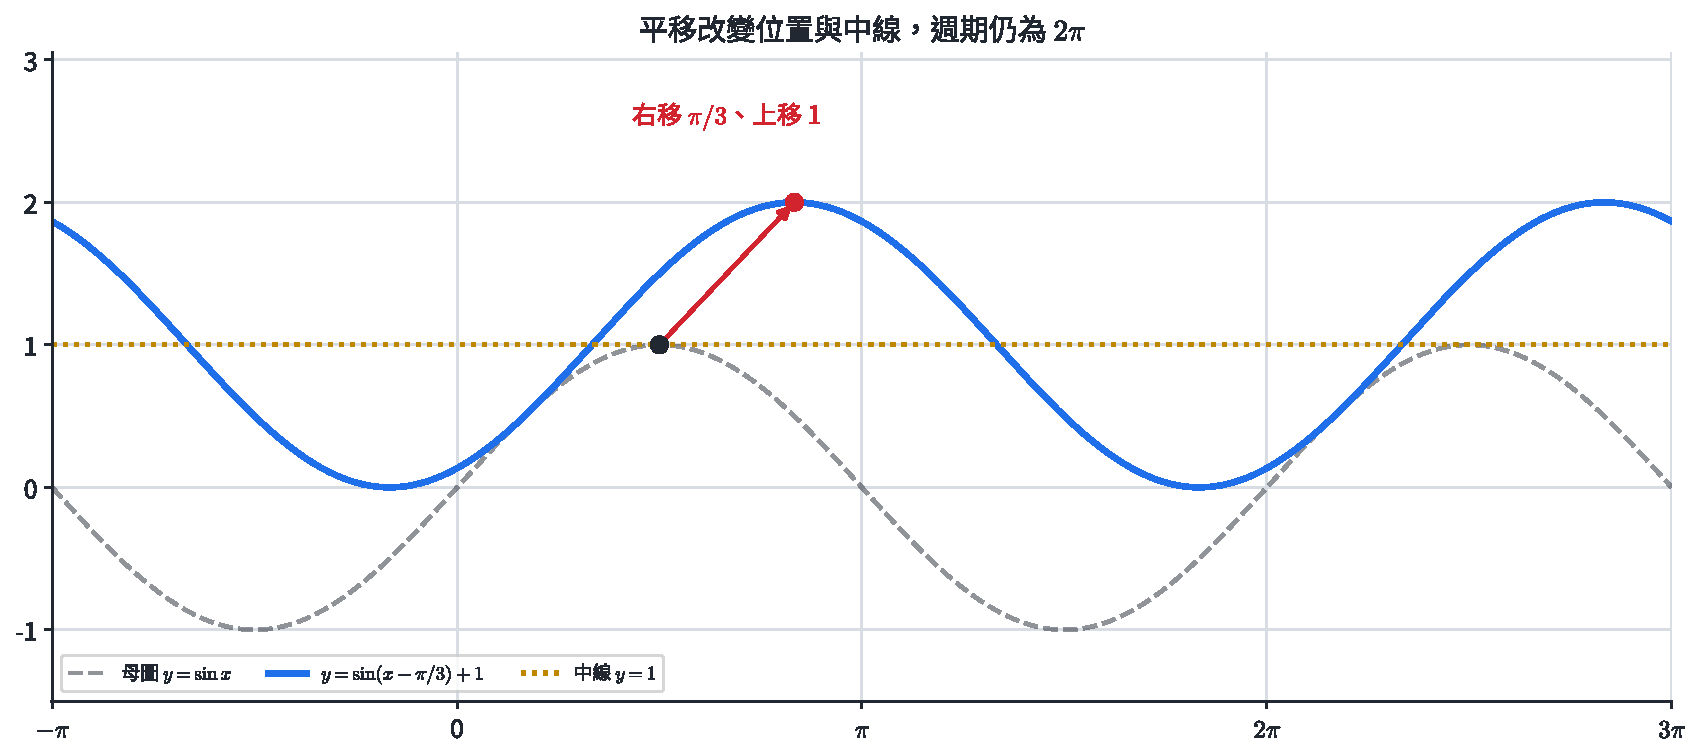
\includegraphics[width=0.96\linewidth,height=\textheight,keepaspectratio,alt={黑點經右移與上移到達紅點，母圖與變換後圖形保留相同週期}]{assets/數B3-1-正弦平移伸縮.pdf}
\caption{黑點經右移與上移到達紅點，母圖與變換後圖形保留相同週期}
\end{figure}

圖中的箭頭把母圖最高點 \((\pi/2,1)\) 移到 \((5\pi/6,2)\)；橫坐標增加 \(\pi/3\)、縱坐標增加 \(1\)，與公式中的水平、鉛直平移一致。

綜合後得到週期模型

\[
y=d+A\sin\bigl(B(x-C)\bigr),\qquad A>0,\ B>0,\ d,C\in\mathbb R.
\]

四個參數的意義為

\[
\text{中線}=d,\qquad
\text{振幅}=A,\qquad
\text{週期 }T=\frac{2\pi}{B},\qquad
\text{向右平移}=C.
\]

值域為 \([d-A,d+A]\)。週期公式可由內角推得：當 \(x\) 增加 \(T\)，正弦內角增加 \(2\pi\)，所以

\[
B(x+T-C)-B(x-C)=BT=2\pi,
\]

因此 \(T=2\pi/B\)。

母圖上的點 \((u,\sin u)\) 經變換後成為

\[
\left(C+\frac{u}{B},\ d+A\sin u\right).
\]

這個點對應公式能精確放置向上穿越中線、最高點、向下穿越中線與最低點。

\begin{figure}
\centering
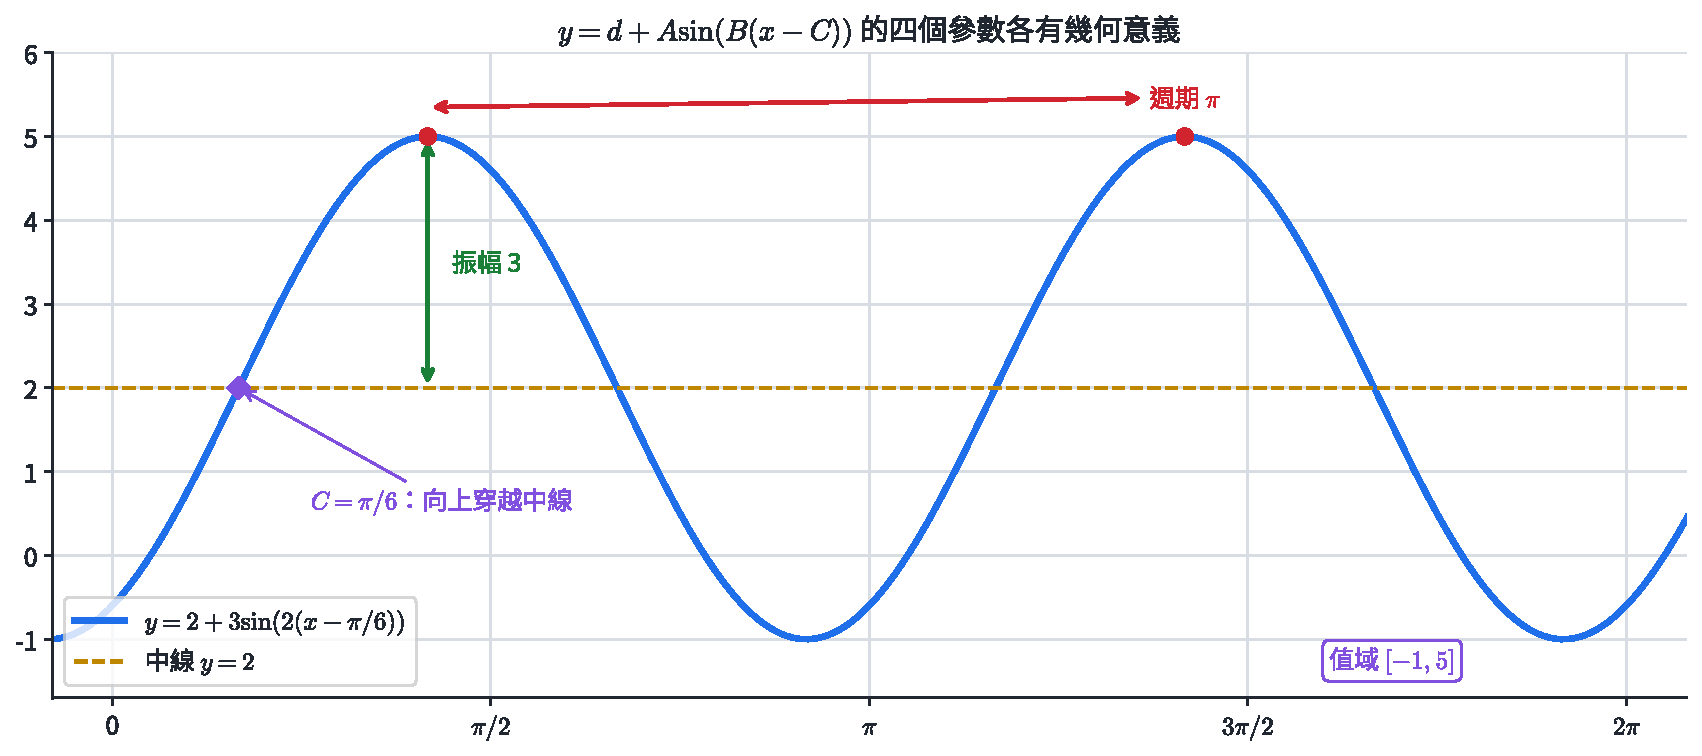
\includegraphics[width=0.96\linewidth,height=\textheight,keepaspectratio,alt={相位點、中線到最高點的振幅，以及相鄰最高點間的週期}]{assets/數B3-1-週期模型參數.pdf}
\caption{相位點、中線到最高點的振幅，以及相鄰最高點間的週期}
\end{figure}

圖中 \(x=C=\pi/6\) 是向上穿越中線的位置；同一個相位狀態經過一個週期後再次出現。振幅由中線量到最高點，週期由相鄰最高點的水平距離量得。

\subsection{5.2 從情境資料決定參數}\label{ux5f9eux60c5ux5883ux8cc7ux6599ux6c7aux5b9aux53c3ux6578}

若週期資料的最大值是 \(M\)、最小值是 \(m\)，則

\[
d=\frac{M+m}{2},\qquad A=\frac{M-m}{2}.
\]

若一次循環需要 \(T\) 個時間單位，則 \(B=2\pi/T\)。最後使用一個已知狀態決定 \(C\)。最方便的狀態通常是：向上穿越中線、到達最高點、向下穿越中線或到達最低點。

若 \(x\) 是時間，頻率 \(f\) 表示每單位時間完成的循環數：

\[
f=\frac1T=\frac{B}{2\pi}.
\]

\subsection{例 15｜讀出正弦函數的全部參數}\label{ux4f8b-15ux8b80ux51faux6b63ux5f26ux51fdux6578ux7684ux5168ux90e8ux53c3ux6578}

分析

\[
y=2+3\sin\left(2\left(x-\frac\pi6\right)\right).
\]

由式子讀出 \(d=2,A=3,B=2,C=\pi/6\)。因此中線為 \(y=2\)，振幅為 \(3\)，值域為 \([-1,5]\)，基本週期為

\[
T=\frac{2\pi}{2}=\pi,
\]

圖形向右平移 \(\pi/6\)。最高點發生在

\[
2\left(x-\frac\pi6\right)=\frac\pi2+2k\pi,
\]

即

\[
x=\frac{5\pi}{12}+k\pi.
\]

\subsection{例 16｜由圖形特徵建立模型}\label{ux4f8b-16ux7531ux5716ux5f62ux7279ux5fb5ux5efaux7acbux6a21ux578b}

某週期量最大值為 \(3\)、最小值為 \(-5\)，週期為 \(6\)；在 \(x=2\) 時向上穿越中線。建立一個正弦模型。

\[
d=\frac{3+(-5)}2=-1,\qquad
A=\frac{3-(-5)}2=4,\qquad
B=\frac{2\pi}{6}=\frac\pi3.
\]

向上穿越中線對應正弦內角 \(0\)，故取 \(C=2\)：

\[
y=-1+4\sin\left(\frac\pi3(x-2)\right).
\]

代入 \(x=2\) 得 \(y=-1\)，接著進入上升段；模型狀態與題目一致。

\subsection{例 17｜聲波的週期與頻率}\label{ux4f8b-17ux8072ux6ce2ux7684ux9031ux671fux8207ux983bux7387}

聲波

\[
y=\sin(880\pi t)
\]

的內角係數為 \(B=880\pi\)，所以

\[
T=\frac{2\pi}{880\pi}=\frac1{440}\text{ 秒},\qquad
f=440\text{ Hz}.
\]

另一聲波 \(y=\sin(1760\pi t)\) 的頻率為 \(880\) Hz，週期為 \(1/880\) 秒。頻率加倍時，同一秒內完成的循環數加倍，週期減半。

\begin{figure}
\centering
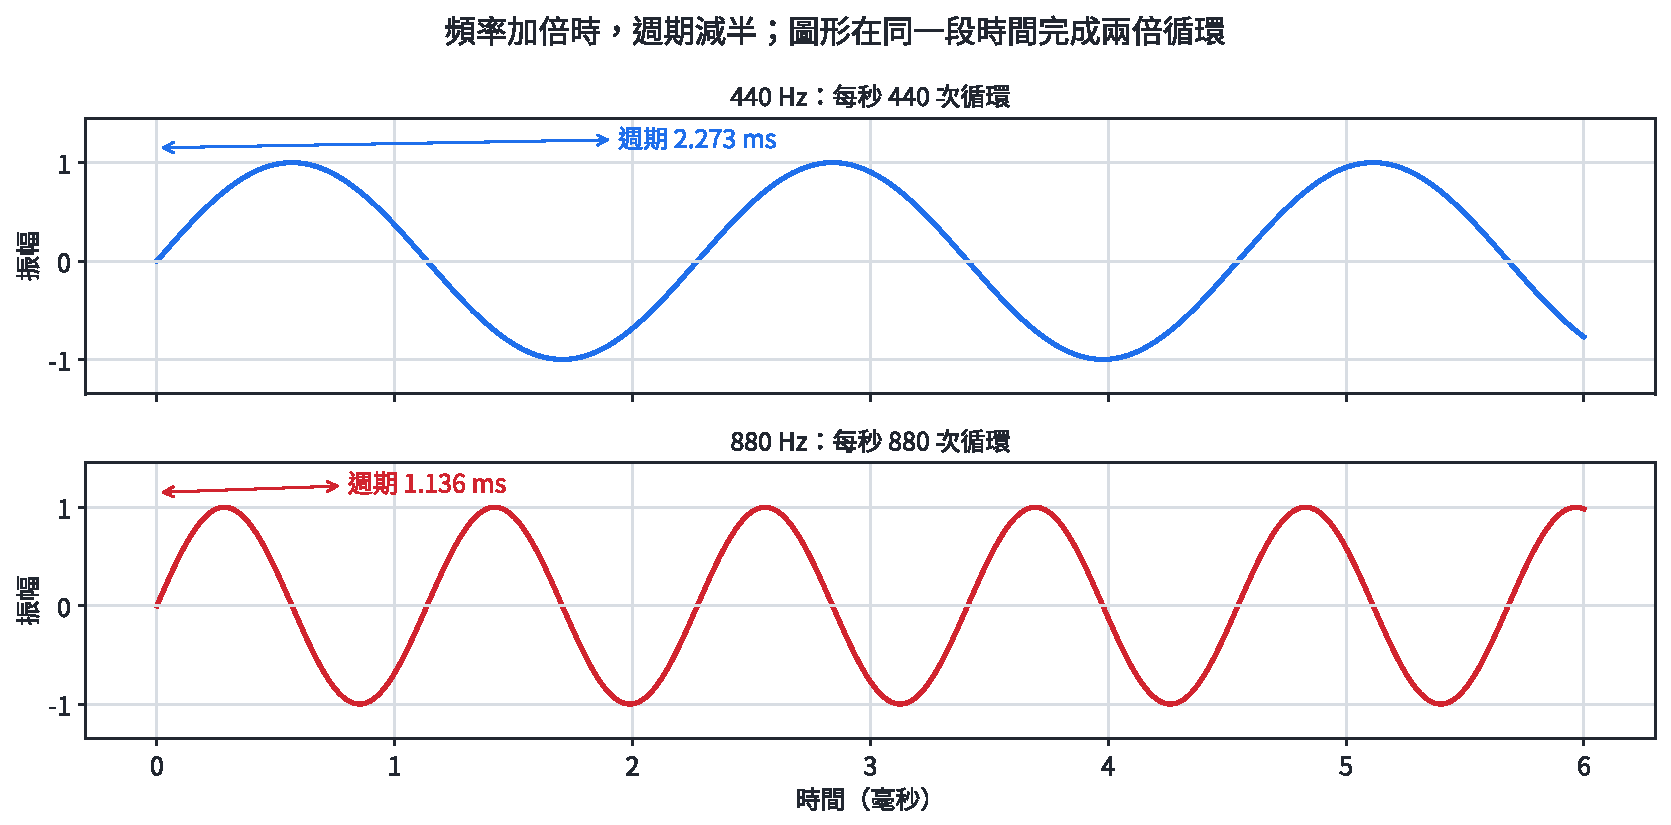
\includegraphics[width=0.95\linewidth,height=\textheight,keepaspectratio,alt={440 Hz 與 880 Hz 聲波的週期比較}]{assets/數B3-1-聲波週期與頻率.pdf}
\caption{440 Hz 與 880 Hz 聲波的週期比較}
\end{figure}

\subsection{例 18｜摩天輪高度模型}\label{ux4f8b-18ux6469ux5929ux8f2aux9ad8ux5ea6ux6a21ux578b}

摩天輪半徑為 \(18\) 公尺，圓心離地 \(20\) 公尺，每 \(15\) 分鐘轉一圈。乘客在 \(t=0\) 從最低點出發。

中線 \(d=20\)，振幅 \(A=18\)，週期 \(T=15\)，所以 \(B=2\pi/15\)。正弦函數在內角 \(-\pi/2\) 時為最低值。令 \(t=0\) 對應 \(-\pi/2\)，得到

\[
h(t)=20+18\sin\left(\frac{2\pi}{15}\left(t-\frac{15}{4}\right)\right).
\]

\(t=5\) 時，內角為 \(\pi/6\)，故

\[
h(5)=20+18\cdot\frac12=29\text{ m}.
\]

同一圈中下降段的 \(t=10\) 也有高度 \(29\) 公尺，因為此時內角為 \(5\pi/6\)。

圓心高 \(20\) 公尺、半徑 \(18\) 公尺，所以最低點仍離地 \(20-18=2\) 公尺。圖中的 \(t=5\) 與 \(t=10\) 落在同一條 \(h=29\) 公尺水平線上，對應上升段與下降段的兩個時刻。

\begin{figure}
\centering
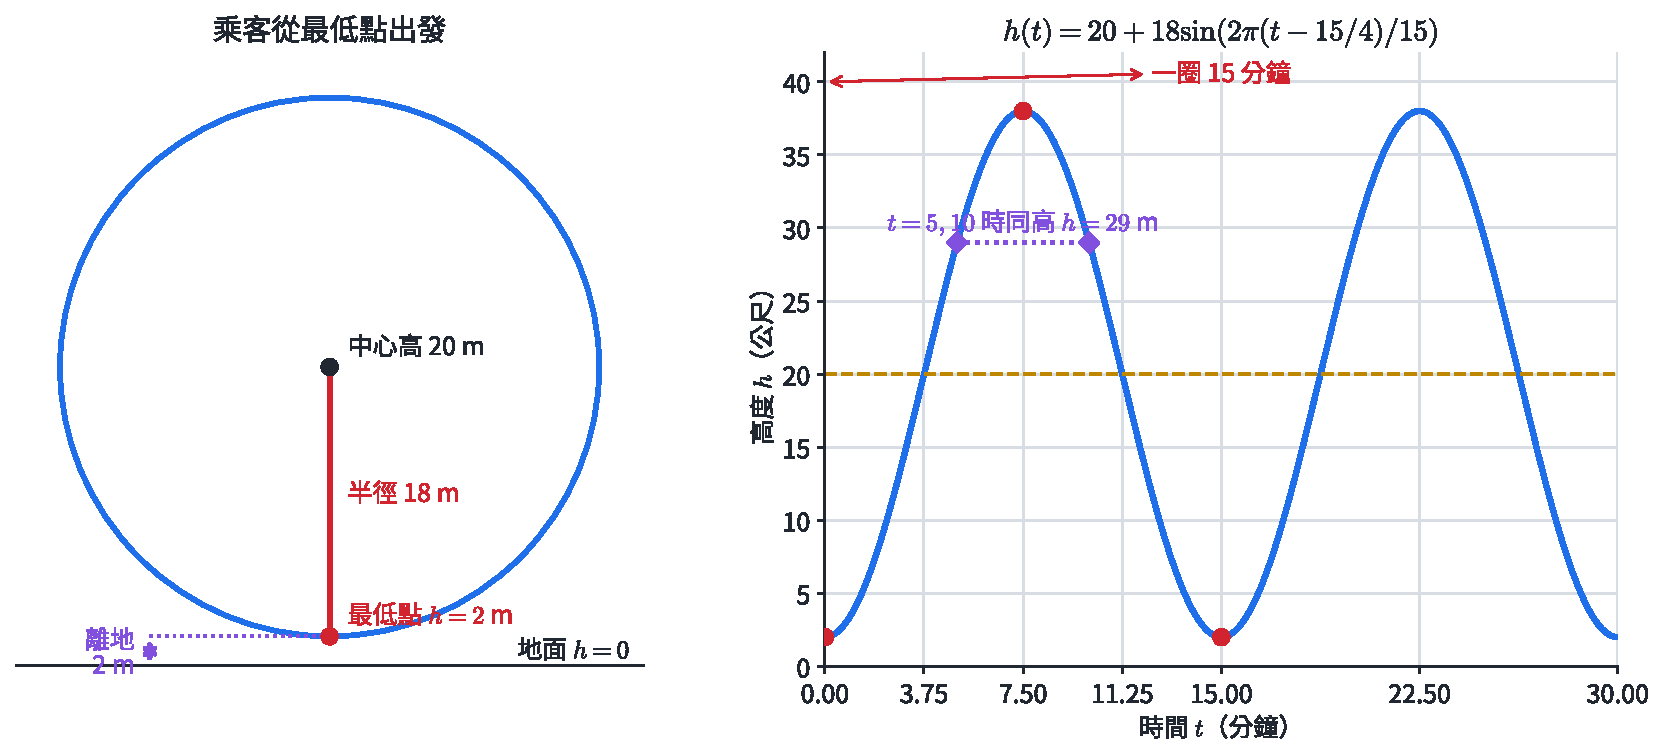
\includegraphics[width=0.97\linewidth,height=\textheight,keepaspectratio,alt={最低點離地 2 公尺，且上升與下降各有一個高度 29 公尺的時刻}]{assets/數B3-1-摩天輪模型.pdf}
\caption{最低點離地 2 公尺，且上升與下降各有一個高度 29 公尺的時刻}
\end{figure}

\subsection{例 19｜由最高、最低與發生時間擬合日溫模型}\label{ux4f8b-19ux7531ux6700ux9ad8ux6700ux4f4eux8207ux767cux751fux6642ux9593ux64ecux5408ux65e5ux6eabux6a21ux578b}

某日溫度近似每 \(24\) 小時循環，最高溫 \(32^\circ\)C 出現在 \(t=14\)，最低溫 \(20^\circ\)C。建立模型並求 \(t=8\) 的預測溫度。

\[
d=\frac{32+20}{2}=26,\qquad A=\frac{32-20}{2}=6,\qquad
B=\frac{2\pi}{24}=\frac\pi{12}.
\]

最高點比向上穿越中線晚四分之一週期，也就是 \(6\) 小時。因此向上穿越中線的時刻為 \(8\)，可取

\[
T(t)=26+6\sin\left(\frac\pi{12}(t-8)\right).
\]

代入 \(t=8\) 得 \(T(8)=26^\circ\)C。這是由單日極值建立的主要趨勢；雲量、風向與降雨會形成觀測值和曲線之間的差異。

\subsection{5.3 分節練習}\label{ux5206ux7bc0ux7df4ux7fd2-4}

\begin{enumerate}
\def\labelenumi{\arabic{enumi}.}
\tightlist
\item
  求 \(y=-2+5\sin\left(3\left(x+\dfrac\pi6\right)\right)\) 的中線、振幅、基本週期、水平平移與值域。
\item
  函數 \(y=7+4\sin(\pi t/5)\) 的基本週期為何？列出 \([0,20]\) 內達最高值的時刻。
\item
  母圖 \(y=\sin u\) 的最高點 \((\pi/2,1)\) 經變換成 \(y=3+2\sin\left(\dfrac12(x-\pi)\right)\) 上的哪一點？
\item
  某週期量的中線為 \(3\)、振幅為 \(2\)、週期為 \(8\)，在 \(t=1\) 向上穿越中線。建立一個正弦模型。
\item
  聲波 \(y=\sin(1200\pi t)\) 的頻率與週期為何？
\item
  摩天輪半徑 \(12\) 公尺、圓心離地 \(14\) 公尺，每 \(8\) 分鐘一圈；乘客從最低點出發。建立正弦高度模型，並求最高點時刻及 \(t=1\) 的高度。
\end{enumerate}

\subsection{5.4 分節練習解析}\label{ux5206ux7bc0ux7df4ux7fd2ux89e3ux6790-4}

\begin{enumerate}
\def\labelenumi{\arabic{enumi}.}
\tightlist
\item
  改寫括號為 \(x-(-\pi/6)\)，得到 \(d=-2,A=5,B=3,C=-\pi/6\)。中線為 \(y=-2\)，振幅為 \(5\)，週期為 \(2\pi/3\)，向左平移 \(\pi/6\)，值域為 \([-7,3]\)。
\item
  \(B=\pi/5\)，故 \(T=2\pi/(\pi/5)=10\)。最高點滿足 \(\pi t/5=\pi/2+2k\pi\)，所以 \(t=2.5+10k\)。在 \([0,20]\) 內為 \(t=2.5,12.5\)。
\item
  點對應公式給出
  \[x=\pi+\frac{\pi/2}{1/2}=2\pi,\qquad y=3+2(1)=5.\]
  所以對應點是 \((2\pi,5)\)。
\item
  \(d=3,A=2,B=2\pi/8=\pi/4\)，向上穿越中線的時刻可作為 \(C\)，所以
  \[y=3+2\sin\left(\frac\pi4(t-1)\right).\]
\item
  \(B=1200\pi=2\pi f\)，所以 \(f=600\) Hz，
  \[T=\frac1{600}\text{ 秒}.\]
\item
  \(d=14,A=12,B=2\pi/8=\pi/4\)。最低點比向上穿越中線早四分之一週期，即 \(2\) 分鐘，因此
  \[h(t)=14+12\sin\left(\frac\pi4(t-2)\right).\]
  最高點在 \(t=4\) 分鐘。\(t=1\) 時
  \[h(1)=14+12\sin\left(-\frac\pi4\right)=14-6\sqrt2\approx5.51\text{ m}.\]
\end{enumerate}

週期模型廣泛用於聲學、機械振動、日照、溫度與水位資料。參數先由幾何或資料決定，再用已知狀態校準相位；最後把預測值放回實際單位與合理範圍檢查。

\section{6. 章末代表題與分層練習}\label{ux7ae0ux672bux4ee3ux8868ux984cux8207ux5206ux5c64ux7df4ux7fd2}

\subsection{A. 基礎與概念}\label{a.-ux57faux790eux8207ux6982ux5ff5}

\begin{enumerate}
\def\labelenumi{\arabic{enumi}.}
\tightlist
\item
  將 \(330^\circ\) 化為弧度，並將 \(-5\pi/8\) 化為度數。
\item
  求 \(41\pi/6\) 在 \([0,2\pi)\) 的同界角、所在象限與正弦值。
\item
  半徑 \(9\) 公分、圓心角 \(4\pi/9\) 的扇形，求弧長與面積。
\item
  一扇形弧長 \(12\) 公分、面積 \(30\) 平方公分，求半徑與圓心角。
\item
  序列由 \(A,B,C,D,E,F\) 六個符號依序循環。第一項為 \(A\)，求第 \(1000\) 項。
\item
  說明函數 \(f(x)=5-2\sin(4x)\) 的一個週期，並求基本週期。
\end{enumerate}

\subsection{B. 圖形與模型}\label{b.-ux5716ux5f62ux8207ux6a21ux578b}

\begin{enumerate}
\def\labelenumi{\arabic{enumi}.}
\setcounter{enumi}{6}
\tightlist
\item
  在 \([-\pi,3\pi]\) 列出 \(y=\sin x\) 的全部零點、最高點與最低點橫坐標。
\item
  在 \([0,2\pi]\) 解 \(\sin x=1/2\)。
\item
  在 \([0,2\pi]\) 解 \(\sin x<-\sqrt3/2\)。
\item
  求 \(y=1+3\sin\left(\dfrac12(x-\pi)\right)\) 的中線、振幅、基本週期、水平平移與值域。
\item
  一週期模型最大值為 \(18\)、最小值為 \(6\)、週期為 \(10\)，在 \(t=3\) 向上穿越中線。建立正弦模型。
\item
  聲波 \(s(t)=0.8\sin(1000\pi t)\) 的振幅、頻率與週期為何？
\end{enumerate}

\subsection{C. 跨節整合}\label{c.-ux8de8ux7bc0ux6574ux5408}

\begin{enumerate}
\def\labelenumi{\arabic{enumi}.}
\setcounter{enumi}{12}
\tightlist
\item
  分針長 \(15\) 公分。從 2:10 到 2:46，求分針轉角、針尖路程與掃過面積。
\item
  一環形扇面外半徑 \(24\) 公分、內半徑 \(10\) 公分，展開角為 \(150^\circ\)。求面積與邊界周長。
\item
  一座摩天輪直徑 \(30\) 公尺，圓心離地 \(18\) 公尺，每 \(12\) 分鐘一圈。乘客在 \(t=0\) 從最低點出發。建立正弦高度模型，求第一次到達最高點的時刻，並求 \(t=2\) 的高度。
\item
  某地連續四次高水位時刻為 \(1.0,13.6,26.1,38.5\) 小時，相應水位為 \(4.7,4.9,4.6,4.8\) 公尺；鄰近三次低水位平均為 \(0.8\) 公尺。估計週期、中線與振幅，取 \(t=1.0\) 為最高點建立正弦模型，並說明模型對下一次高水位時刻與水位的預測。
\end{enumerate}

\section{7. 章末分層練習詳解}\label{ux7ae0ux672bux5206ux5c64ux7df4ux7fd2ux8a73ux89e3}

\begin{enumerate}
\def\labelenumi{\arabic{enumi}.}
\tightlist
\item
  \[330^\circ=330\cdot\frac\pi{180}=\frac{11\pi}{6}.\]
  \[-\frac{5\pi}{8}\cdot\frac{180}{\pi}{}^\circ=-112.5^\circ.\]
\item
  減去三圈：
  \[\frac{41\pi}{6}-6\pi=\frac{5\pi}{6}.\]
  位於第二象限，且 \(\sin(41\pi/6)=1/2\)。
\item
  \[s=9\cdot\frac{4\pi}{9}=4\pi\text{ cm},\]
  \[A=\frac12(9)^2\frac{4\pi}{9}=18\pi\text{ cm}^2.\]
\item
  由 \(A=rs/2\)，
  \[30=\frac12r(12)\quad\Rightarrow\quad r=5\text{ cm}.\]
  再由 \(s=r\theta\)，得到 \(\theta=12/5\) 弧度。
\item
  基本週期為 \(6\)。\(1000-1=999\)，除以 \(6\) 餘 \(3\)，故第 \(1000\) 項是循環索引 \(3\)，也就是第四個符號 \(D\)。
\item
  對 \(T=\pi/2\)，
  \[f\left(x+\frac\pi2\right)=5-2\sin(4x+2\pi)=f(x).\]
  所以 \(\pi/2\) 是週期；正弦內角係數為 \(4\)，基本週期為 \(2\pi/4=\pi/2\)。
\item
  零點 \(x=k\pi\)，在區間內為
  \[-\pi,0,\pi,2\pi,3\pi.\]
  最高點橫坐標為 \(\pi/2,5\pi/2\)；最低點橫坐標為 \(-\pi/2,3\pi/2\)。
\item
  單位圓縱坐標為 \(1/2\) 的角位於第一、第二象限：
  \[x=\frac\pi6,\frac{5\pi}{6}.\]
\item
  邊界解為 \(x=4\pi/3,5\pi/3\)。正弦曲線在兩點之間低於 \(-\sqrt3/2\)，故
  \[\frac{4\pi}{3}<x<\frac{5\pi}{3}.\]
\item
  \(d=1,A=3,B=1/2,C=\pi\)。中線 \(y=1\)，振幅 \(3\)，週期
  \[T=\frac{2\pi}{1/2}=4\pi,\]
  向右平移 \(\pi\)，值域為 \([-2,4]\)。
\item
  \[d=\frac{18+6}{2}=12,\qquad A=\frac{18-6}{2}=6,\qquad
  B=\frac{2\pi}{10}=\frac\pi5.\]
  \(t=3\) 向上穿越中線，故
  \[y=12+6\sin\left(\frac\pi5(t-3)\right).\]
\item
  函數外係數給出振幅 \(0.8\)。內角係數 \(B=1000\pi\)，所以
  \[f=\frac{B}{2\pi}=500\text{ Hz},\qquad T=\frac1{500}\text{ 秒}.\]
\item
  經過 \(36\) 分鐘，占一圈的 \(3/5\)，所以
  \[\theta=2\pi\cdot\frac35=\frac{6\pi}{5}.\]
  針尖路程為
  \[s=15\cdot\frac{6\pi}{5}=18\pi\text{ cm}.\]
  掃過面積為
  \[A=\frac12(15)^2\frac{6\pi}{5}=135\pi\text{ cm}^2.\]
  轉角、弧長與面積都使用同一個時間比例 \(3/5\)。
\item
  \(150^\circ=5\pi/6\)。面積為
  \[A=\frac12(24^2-10^2)\frac{5\pi}{6}
  =\frac{595\pi}{3}\text{ cm}^2.\]
  邊界周長為
  \[P=(24+10)\frac{5\pi}{6}+2(24-10)
  =\frac{85\pi}{3}+28\text{ cm}.\]
\item
  半徑 \(A=15\)，中線高度 \(d=18\)，週期 \(12\)，所以 \(B=\pi/6\)。最低點比向上穿越中線早 \(3\) 分鐘，模型為
  \[h(t)=18+15\sin\left(\frac\pi6(t-3)\right).\]
  從最低點到最高點需半圈，即 \(6\) 分鐘。\(t=2\) 時
  \[h(2)=18+15\sin\left(-\frac\pi6\right)=10.5\text{ m}.\]
  高度範圍為 \([3,33]\) 公尺，計算值落在範圍內。
\item
  三段高水位間隔為 \(12.6,12.5,12.4\) 小時，故
  \[T=\frac{12.6+12.5+12.4}{3}=12.5\text{ 小時}.\]
  四次高水位平均為
  \[M=\frac{4.7+4.9+4.6+4.8}{4}=4.75\text{ m}.\]
  取低水位 \(m=0.8\) 公尺，則
  \[d=\frac{4.75+0.8}{2}=2.775,\qquad
  A=\frac{4.75-0.8}{2}=1.975.\]
  \(t=1.0\) 是最高點。最高點比向上穿越中線晚四分之一週期，故模型可寫成
  \[h(t)=2.775+1.975\sin\left(\frac{2\pi}{12.5}(t+2.125)\right).\]
  模型對前三次後續高水位時刻的預測為 \(13.5,26.0,38.5\) 小時，與觀測相差約 \(0\) 至 \(0.1\) 小時。資料末筆之後的下一次高水位預測為
  \[38.5+12.5=51.0\text{ 小時},\]
  水位為 \(4.75\) 公尺。觀測高水位在 \(4.6\) 至 \(4.9\) 公尺間，呈現單一正弦模型未納入的短期變化。
\end{enumerate}

\section{8. 核心整理}\label{ux6838ux5fc3ux6574ux7406}

\begin{itemize}
\tightlist
\item
  弧度定義：\(\theta=s/r\)；一整圈是 \(2\pi\)。
\item
  換算：度數乘 \(\pi/180\) 得弧度；弧度乘 \(180/\pi\) 得度數。
\item
  扇形：\(s=r\theta\)，\(A=r^2\theta/2=rs/2\)，其中 \(\theta\) 使用弧度。
\item
  週期：\(f(x+T)=f(x)\)；最小正週期是基本週期。
\item
  \(y=\sin x\)：定義域 \(\mathbb R\)、值域 \([-1,1]\)、基本週期 \(2\pi\)，且 \(\sin(-x)=-\sin x\)。
\item
  一般模型 \(y=d+A\sin(B(x-C))\)：中線 \(d\)、振幅 \(A\)、週期 \(2\pi/B\)、向右平移 \(C\)、值域 \([d-A,d+A]\)。
\item
  若最大值為 \(M\)、最小值為 \(m\)，則 \(d=(M+m)/2\)、\(A=(M-m)/2\)。
\item
  時間模型的頻率 \(f=1/T=B/(2\pi)\)。
\item
  實際資料以主要週期建立近似，觀測值和模型值之差保留其他因素的影響。
\end{itemize}


\end{document}
